\documentclass[tikz,border=6pt]{standalone}
\usepackage{xcolor}
\usetikzlibrary{arrows.meta,positioning}

\definecolor{blockblue}{HTML}{4A90D9}
\definecolor{linegray}{HTML}{333333}

\begin{document}
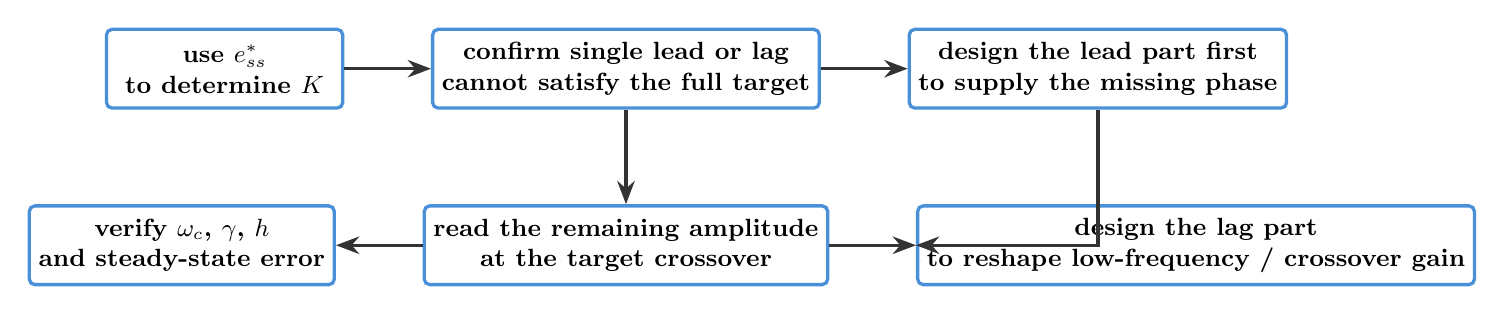
\begin{tikzpicture}[
  >=Stealth,
  line width=1.2pt,
  stage/.style={rectangle, draw=blockblue, rounded corners=2pt, minimum width=3.0cm, minimum height=1.0cm, align=center, font=\small\bfseries},
  flow/.style={->, draw=linegray, line width=1.2pt}
]
  \node[stage] (s1) at (0,0) {use $e_{ss}^\ast$\\to determine $K$};
  \node[stage, right=1.1cm of s1] (s2) {confirm single lead or lag\\cannot satisfy the full target};
  \node[stage, right=1.1cm of s2] (s3) {design the lead part first\\to supply the missing phase};
  \node[stage, below=1.2cm of s2] (s4) {read the remaining amplitude\\at the target crossover};
  \node[stage, right=1.1cm of s4] (s5) {design the lag part\\to reshape low-frequency / crossover gain};
  \node[stage, left=1.1cm of s4] (s6) {verify $\omega_c$, $\gamma$, $h$\\and steady-state error};
  \draw[flow] (s1) -- (s2);
  \draw[flow] (s2) -- (s3);
  \draw[flow] (s2) -- (s4);
  \draw[flow] (s3) |- (s5);
  \draw[flow] (s4) -- (s5);
  \draw[flow] (s4) -- (s6);
\end{tikzpicture}
\end{document}
